% Uncomment:

% \note{Notes on Band 5 robust = -1?}


% During the data analysis of the ALMA images, we noticed a faint source in the background of the images in Bands 5 and 7. These images in Stokes I can be found in Figure \ref{fig: GC_StokesI_BothBands}. From these images we can see that it is the same source seen at both wavelengths. This source is not seen in Bands 4 and 6.


% % ---------------------------------------------------------

% \begin{figure*}[h]
%   \centering
%   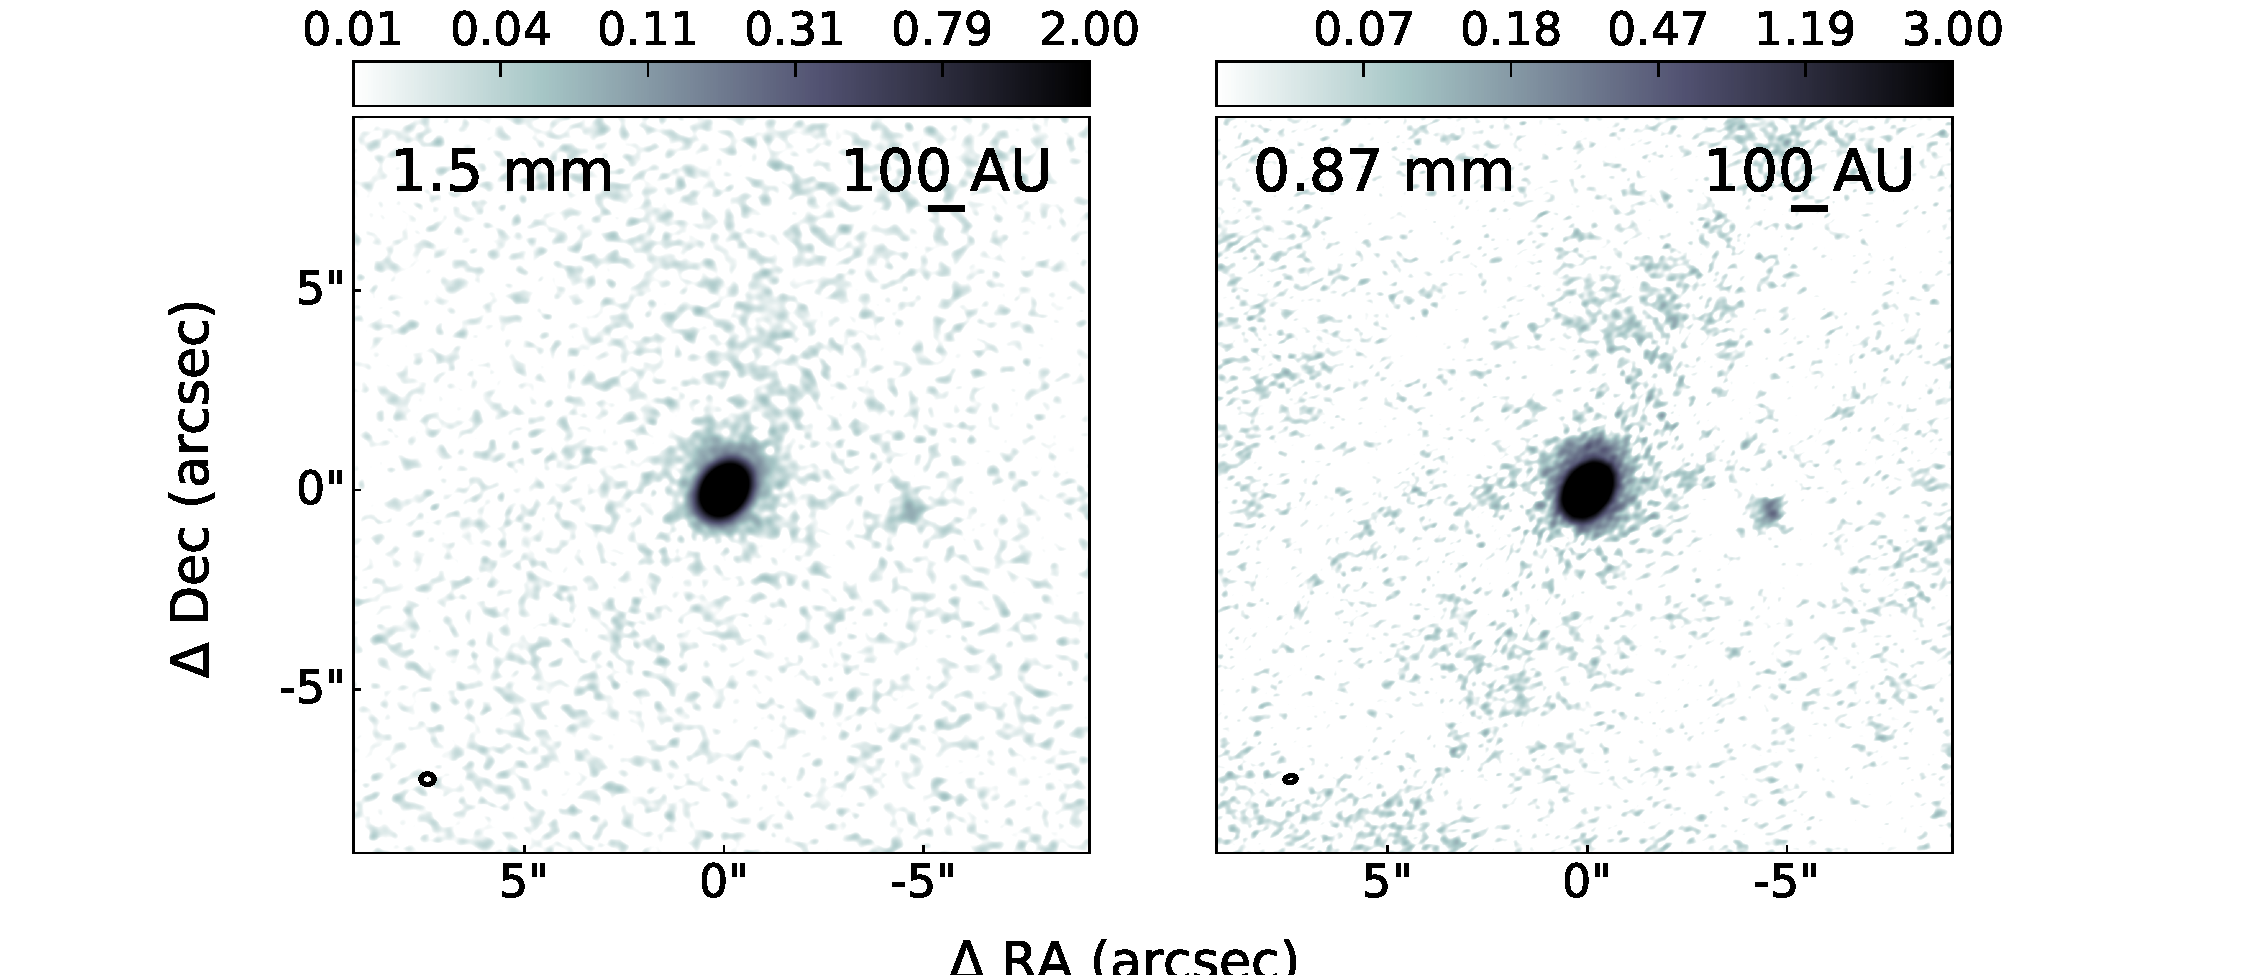
\includegraphics[width=1.1\textwidth]{../IMAGES/WRITEUP/GalaxyContamination/StokesI_BothBands.pdf}
%   \caption{Stokes I images of Band 5 (left) and Band 7 (right) to show the background source to the right of the disk. Note that lowest and highest Stokes I values are cutoff for visualization. Band 5 ranges: (-0.05710974, 79.41323) $\ra$ (0.006, 2) and Band 7 ranges: (-0.14653777, 175.78313) $\ra$ (0.02, 3), all values in mJy and were chosen by eye.  \question{Should I add a marker to show its the exact same location? A circle?}}
%   \label{fig: GC_StokesI_BothBands}
% \end{figure*}




% \begin{figure*}[h]
%   \centering
%   % First figure
%   \begin{minipage}{0.48\textwidth}
%     \centering
%     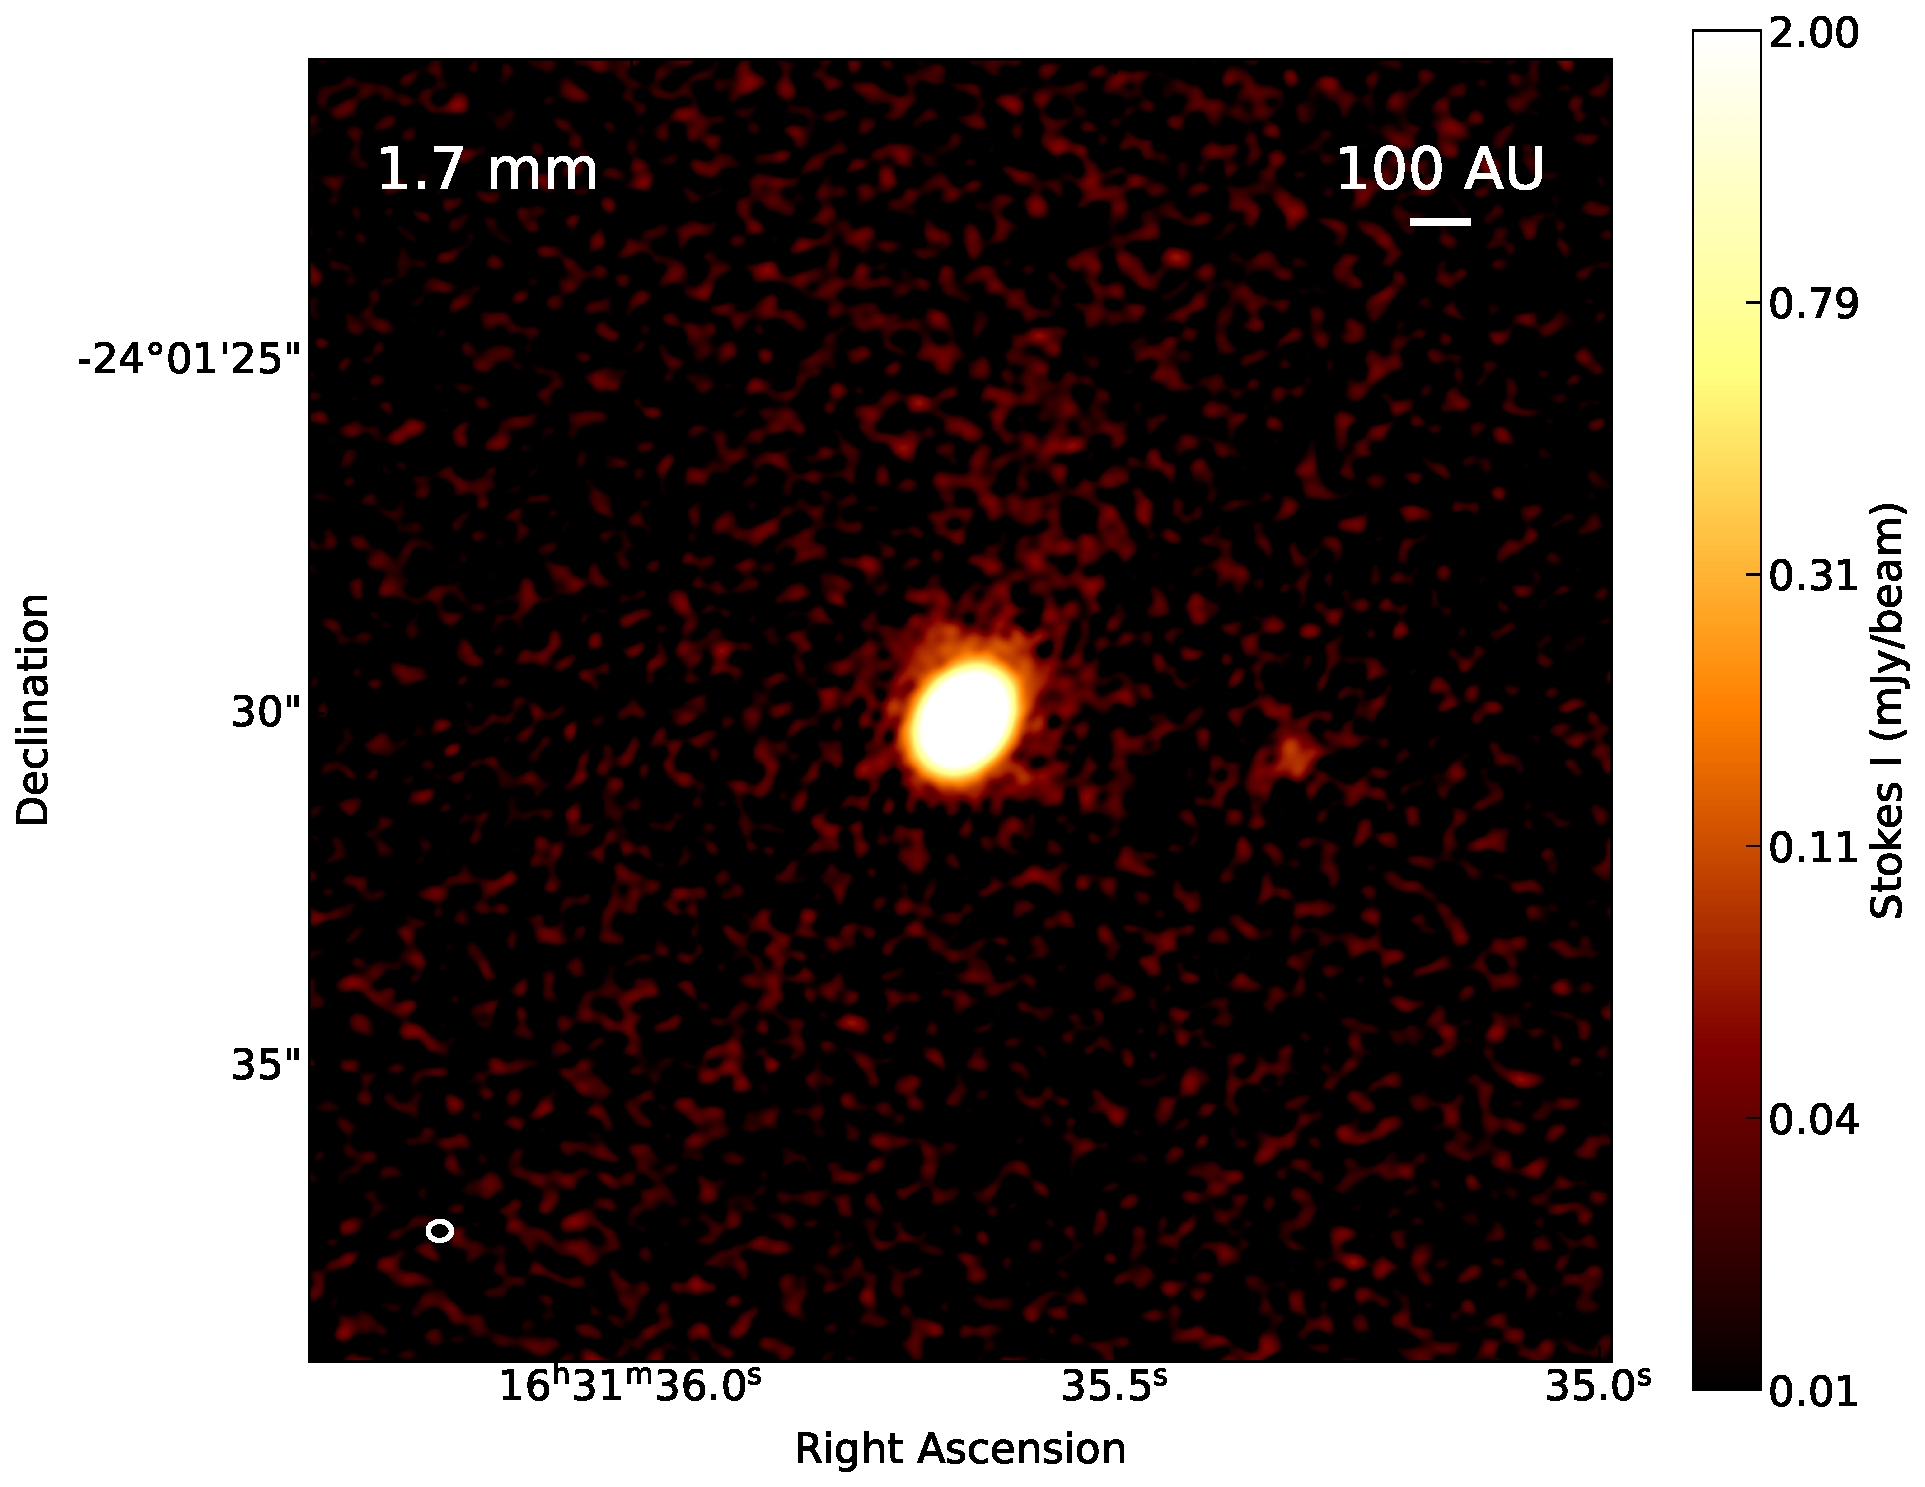
\includegraphics[width=\linewidth]{WRITEUP_AND_IMAGES/IMAGES/WRITEUP/GalaxyContamination/StokesI_BAND5.pdf}
%     \caption{Galaxy Contamination of Band 5. Note that Stokes I is cutoff for visualization.}
%     \label{fig: GC_POLI_Band5}
%   \end{minipage}%
%   \hfill
%   % Second figure
%   \begin{minipage}{0.48\textwidth}
%     \centering
%     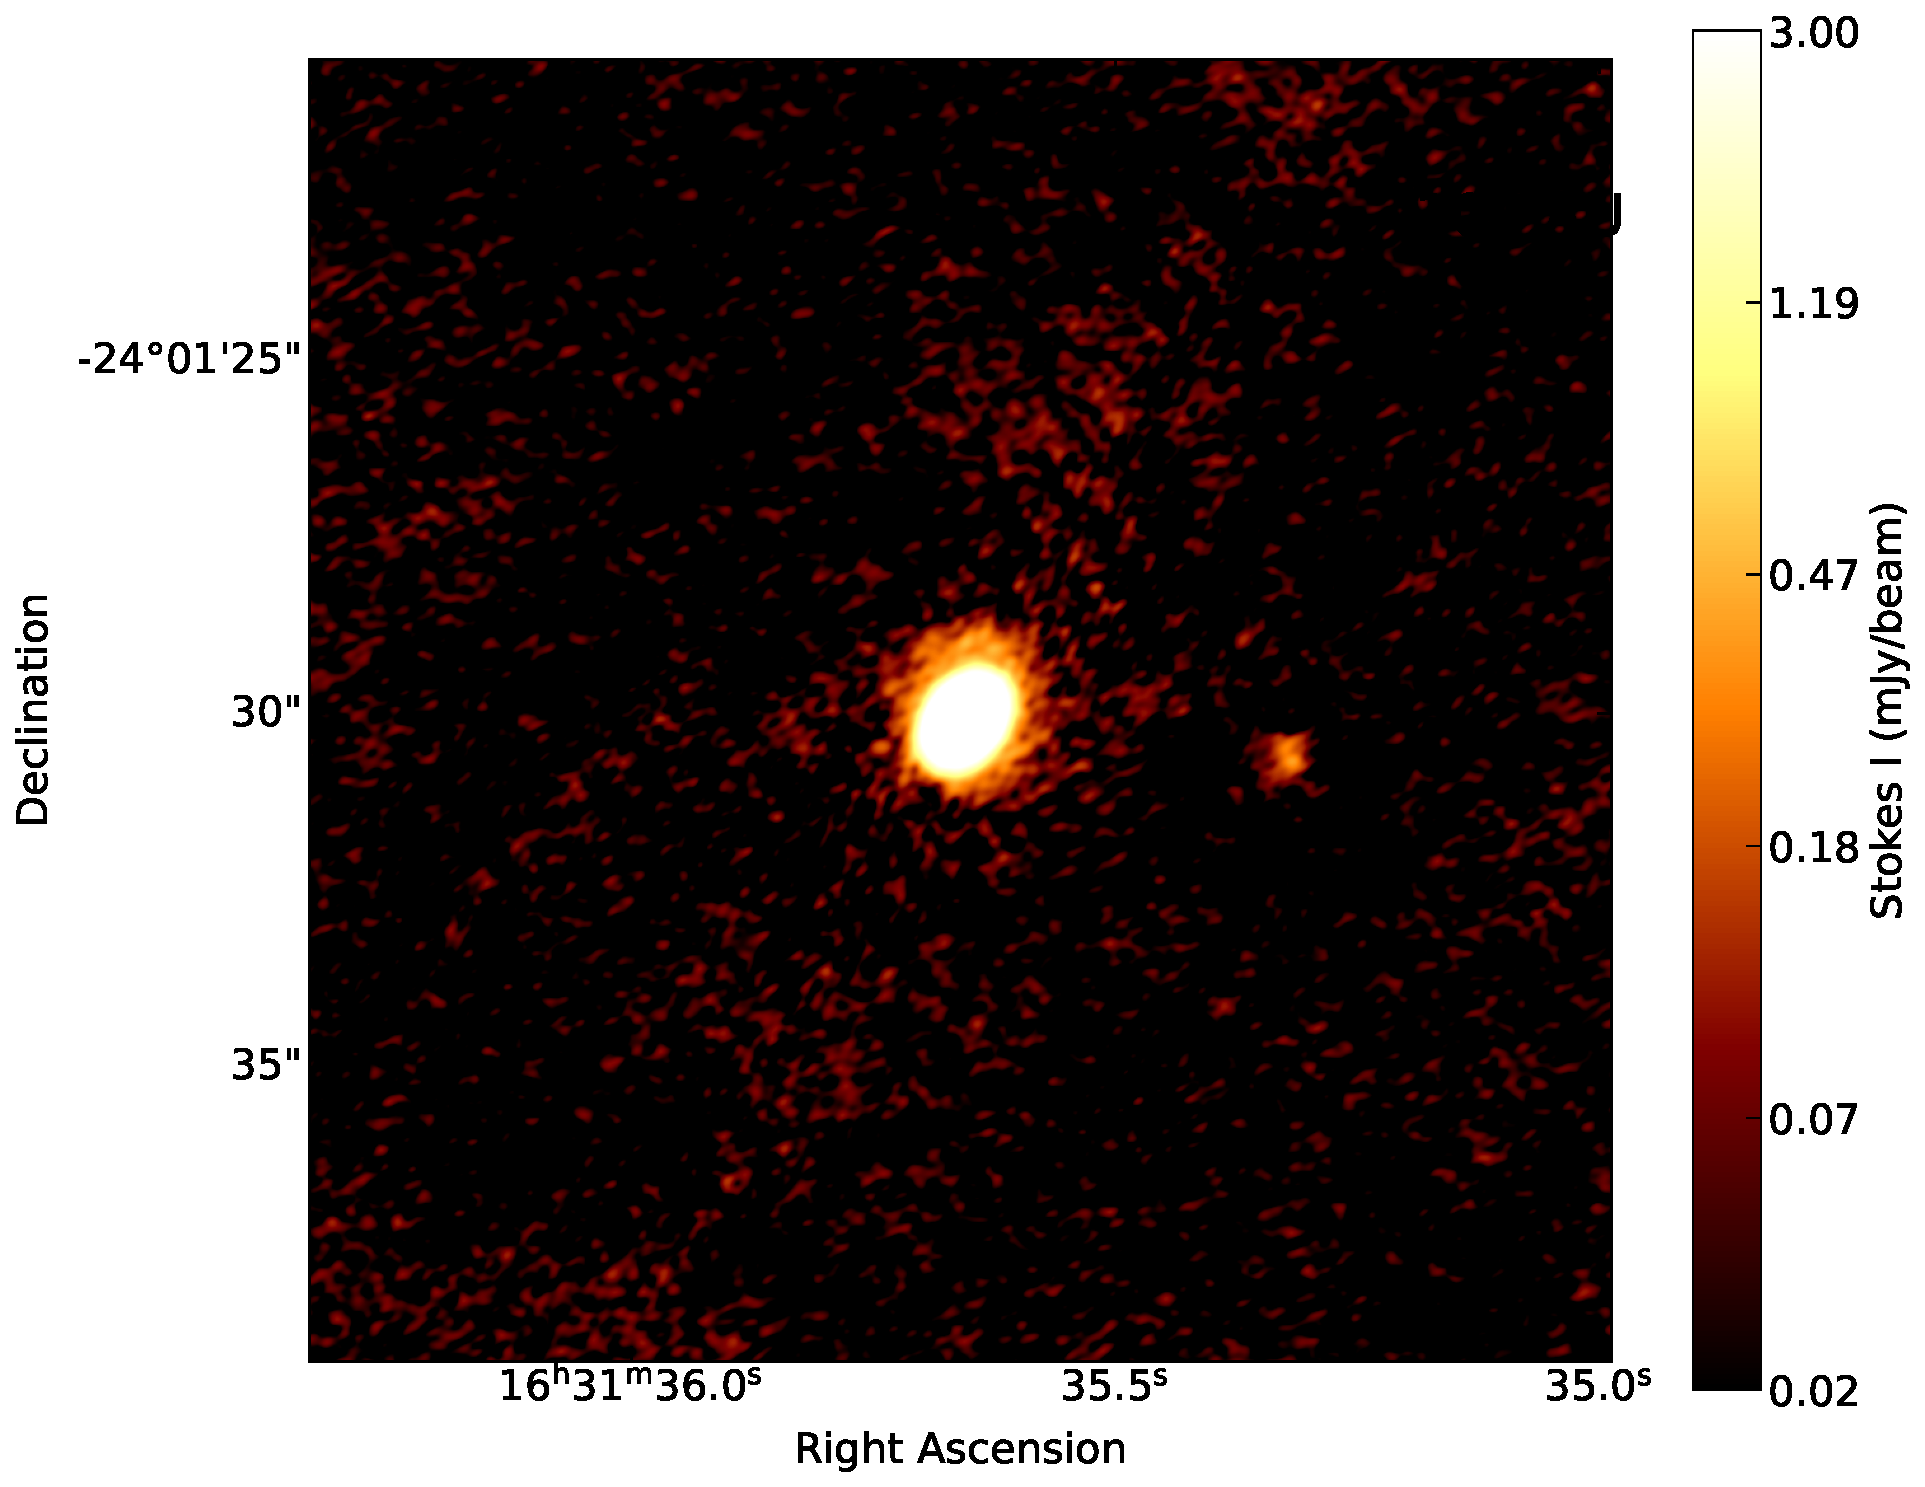
\includegraphics[width=\linewidth]{WRITEUP_AND_IMAGES/IMAGES/WRITEUP/GalaxyContamination/StokesI_BAND7.pdf}
%     \caption{Same as Figure \ref{fig: GC_POLI_Band5}, but for Band 7. Note that Stokes I is cutoff for visualization.}
%     \label{fig: GC_POLI_Band7}
%   \end{minipage}
% \end{figure*}




% ---------------------------------------------------------
% Uncomment:
% It was predicted that this background source may be a background galaxy. The method used to determine the likelihood of detecting a background galaxy was adapted from Section 5.5 in in \citep{sadavoy_dust_2019}. 

% \add{Some sentence about why we can't do this at Band 5.}

% Using \citep{GC_Number_Counts} for the Band 7 number counts, the Schecter function is used to find the number of galaxies per \question{area?}
% \begin{equation}
% \frac{dN}{dS}= N_0 \left(\frac{S}{S_0}\right)^\alpha \exp \left(- \frac{S}{S_0}\right)
% = 923\left(\frac{S}{S_0}\right)^{-1.7} \exp \left(- \frac{S}{S_0}\right),
% \label{eq: GC_Schecter}
% \end{equation}
% \noindent where $N$ is the number of galaxies with intensity $S$, $N_0$ is the normalization factor with units of number per degree squared, $S_0$ is the flux density at the turnover in mJy and $S$ is the intensity of the source, found in our images to be 0.4008985706605 mJy. 


% The signal to noise ratio of the background source is $\sim$9.4391 in Band 7. The distance from the centre of the disk to the source is 4.75 arcsec




% \add{more text here}

% I used the primary beam file provided to replicate Figures 11 and 12 from the paper. I then wanted to use these methods to apply them to my source. 

% The cumulative probability of \add{add here} at $5\sigma$, $9\sigma$ and $20\sigma$ is 58.49\%, 39.89\% and 19.55\%  respectively.



% \begin{figure*}[h]
%   \centering
%   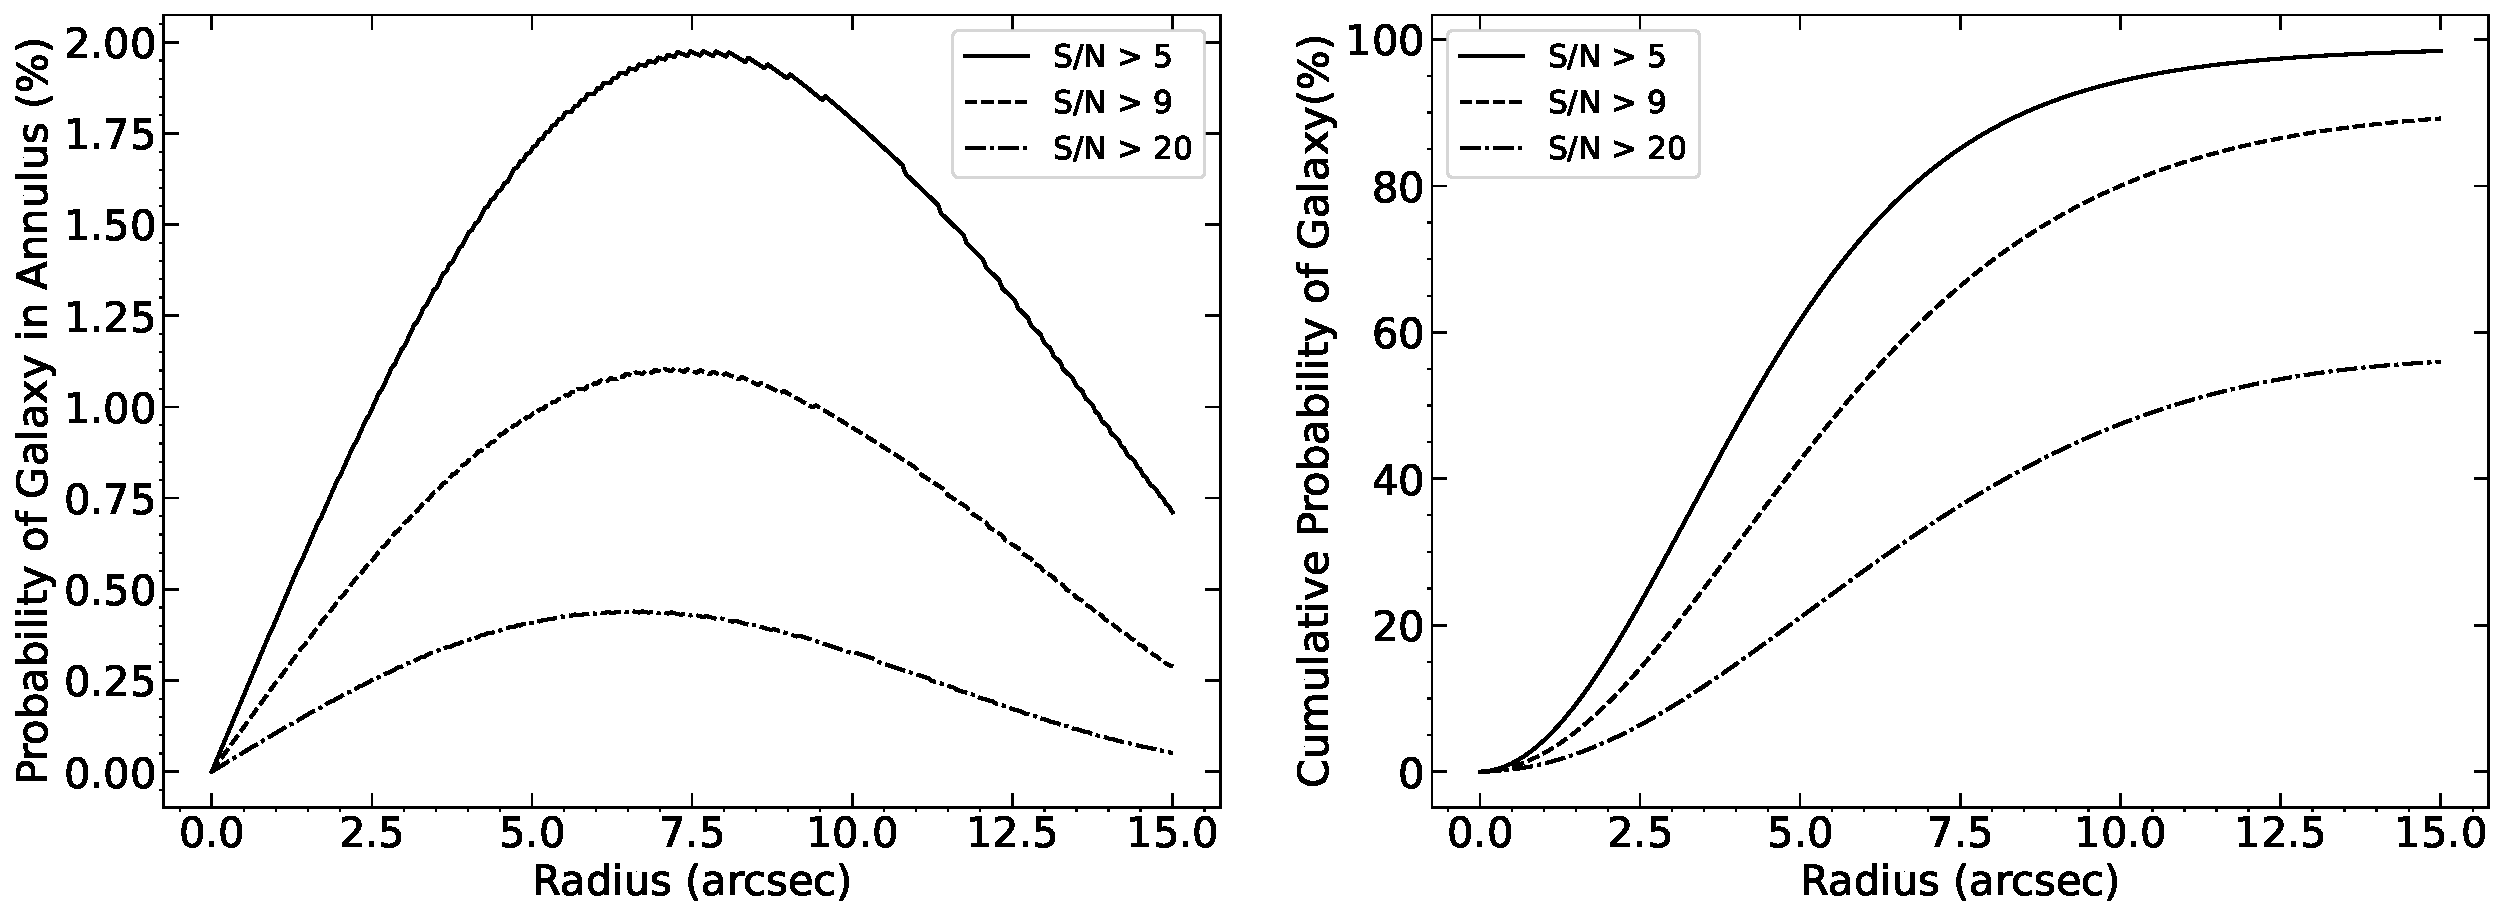
\includegraphics[width=1.1\textwidth]{../IMAGES/WRITEUP/GalaxyContamination/Probabilities_Band7.pdf}
%   \caption{Galaxy contamination for Band 7.}
%   \label{fig: GalaxyContamination_Prob_B7}
% \end{figure*}







% Based on the calculations, the probability of the source being a background galaxy is non-negligible. This result has no direct implications on the results of this project, but rather is a fun side branch result. 


